\section{Discussion}

\subsection{Sobel Edge Detection and Highlighting hair Edges}

Training a neural network can be a very tricky task; a lot of interconnecting parts can easily influence the other. The influence of one simple can be seen from the experimentation in each part of the process. For example, in previous lab exercises, adding or removing just one preprocessing technique can often be seen as futile or irrelevant. Oftentimes, in order to truly leverage preprocessing in the old machine learning models, these techniques need to be combined together. However there is a limit to how much preprocessing one should apply to the data, as introducing more interpolation, variance, or overall noise can be detrimental to the performance of the machine learning model.

Using Table \ref{tab:preprocessing_results} as an example, using Sobel Edge Detection (SED), it reduces overfitting when using the model without any preprocessing methods as the baseline for metrics. While Sobel Edge Detection lowered the training accuracy by around 0.02, overfitting reduced by increasing the accuracy for the validation set by 0.04. Looking at the baseline model, the difference or distance between the accuracy of training and validation sets is much larger than the model that applied SED. 

% TODO: add images of inputs

Sobel Edge Detection allows the CNN to easily capture the features better. Due to SED highlighting the edges in the images, the CNN takes advantage of this modification as it can better look at how the hair flows for each sample. Looking at Figure FIGURE, hairs are no exception to the SED, strands (especially those in the edge of the person's hair) are highlighted and emphasized in the image usually as a white color or something that is in complete contrast with the color assigned to non-edges. Kernels can find these more easily therefore train more easily ultimately leading to a better performance.

\subsection{Data Augmentation and Noise}

Oftentimes data augmentation can be of help with machine learning models to better their performance in the task they were meant to do. But sometimes data augmentation can actually be harmful. Data augmentation can actually increase noise by variating data. Such data augmentations can be good to train a network similar to \cite{kim_adaptive_2021}'s work, however there needs to be a good foundation of having a good network. For a network to be robust to noise, it must be well modelled to be capable of being trained for robustness in the first place. Without a well built model, introducing noise can be detrimental as seen in the experimentations. Table \ref{tab:preprocessing_results} shows the effects of data augmentation to the model, in both cases where it is isolated and combined with Sobel Edge Detection, the model had performed worse. 

\subsection{Overfitting}

Overfitting is a lot easier when dealing with neural networks. Because of the thousandas or millions of little parts that influence each other, mismanagement of a feature can easily lead to overfitting. Looking at the experiments, flattening and using dropout layers, and changing the activation function to LeakyReLU can lead to overfitting without proper "compensation" techniques. In a way to reduce overfitting but maintain the use of flattening and dropout layers, Global Average Pooling can be done first to reduce the chances of overfitting the model.

More layers doesn't always mean more performance; there is the optimal amount of layers that must be identified. Batch Normalizaiton helps in reducing overfitting by applying a transformation that converts inputs to conform in the range $[0, 1]$. According to the tensorflow API, Batch Normalization works by applying the following equation:

\[
  \gamma \cdot \left(\frac{\text{batch} - mean(\text{batch})}{\sqrt{var(\text{batch}) + \epsilon} + \beta}\right)
\]

where the $\epsilon, \gamma, \beta$ are hyperparameters tunable by its users. 

As for LeakyReLU, the dichotomy between training and validation accuracy are as big as ever. Figure \ref{fig:leaky_relu} shows this severe case. Due to this experimentation, we have decided to continue with ReLU instead as the activation function. 

\subsection{Other Models}

Another model was also experimented on to see how it will compare in performance. The U-Net model has done well, reaching as high as 0.70 in accuracy but still converge with the accuracy score of the validation set. However, the convergence of the training and validation scores are only because of chance; if it were any other epoch that were about 10 epochs apart to the current one, the model would've been greatly off. In other words, it lacks consistency, training this with proper regularization or overfitting measures would surely improve performance. However, there is still the need to design our own model from scratch, but as a reference point, this is how a vanilla or plain U-Net would perform in this dataset; adding things such as other activation functions, dropout layers, and such would surely increase performance but that will be outside of the scope for now. 

\subsection{Kernels}

Convolutinal Neural Networks often have multiple kernels and multiple sequences of kernels, We can see how these kernels eventually converge into selecting the most important feature to use for the dense neural network layer. Looking at figure \ref{fig:kernels}, the first convolution of the model were a bit more inconsistent, but looking at the 11th layer, as shown in figure \ref{fig:lower_dimension_kernels}, this convolution layer has 64 output kernels but looking at only three of them, we can see that the kernels weights are more consistent; they all look for the same features or at the very least have resemblance with the other filters.

\begin{figure}[H]
  \centering
  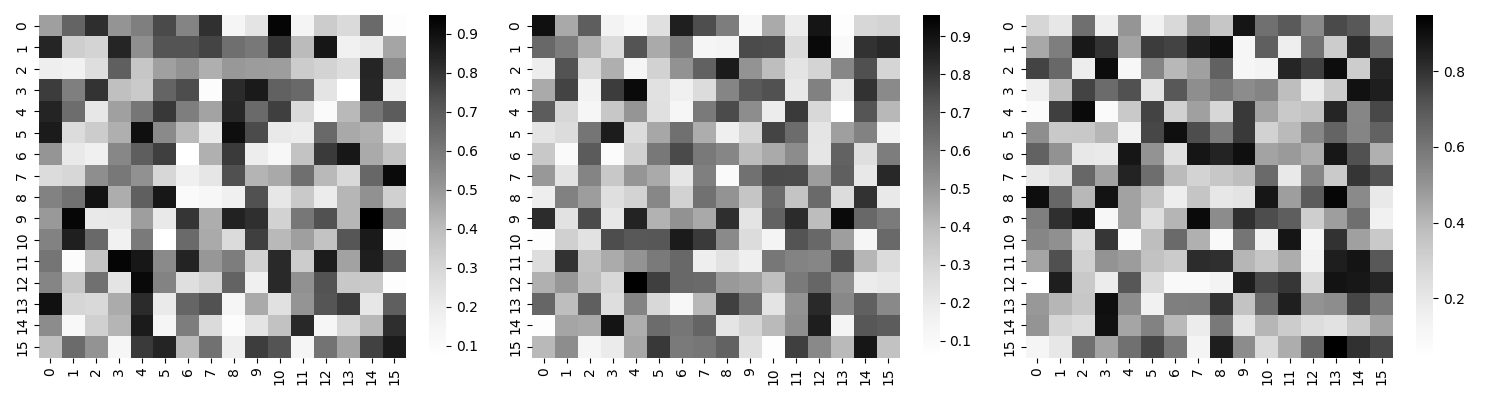
\includegraphics[width=\linewidth]{figures/kernels.png}
  \caption{Filters in the First Convolution Layer}
  \label{fig:kernels}
\end{figure}

\begin{figure}[H]
  \centering
  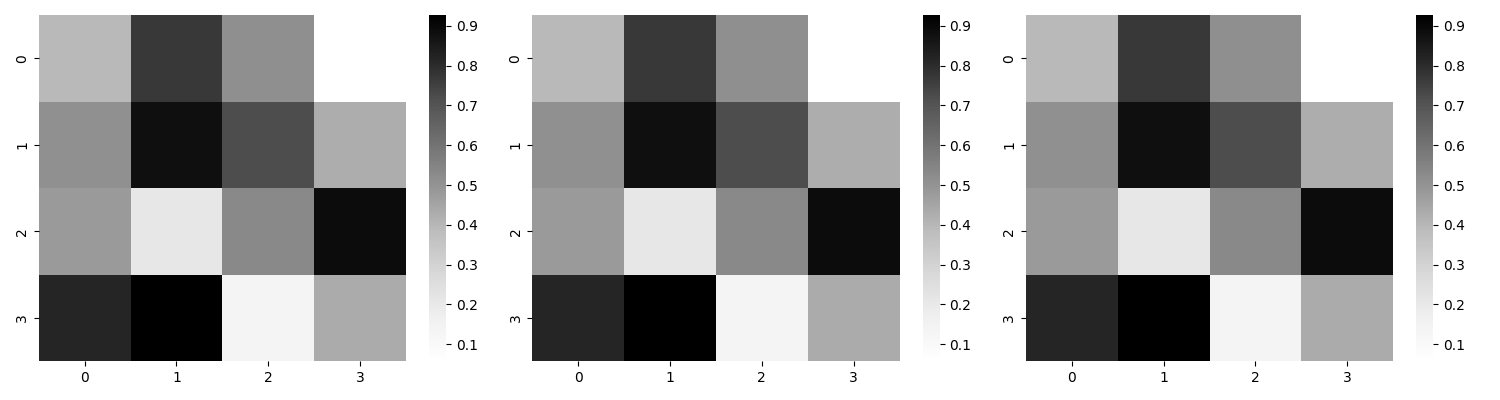
\includegraphics[width=\linewidth]{figures/kernels_lower.png}
  \caption{Filters in the Third Convolution Layer}
  \label{fig:lower_dimension_kernels}
\end{figure}
